\section{Theorie}
\label{sec:Theorie}

\subsection{Zielsetzung}
Die Aufgabe des Versuchs besteht darin, die Schwingungsdauern verschiedener
Schwingungsarten sowie die Schwebungsdauer von jeweils zwei, identischen,
gekoppelten Pendeln zu bestimmen.
\subsection{Theoretische Grundlagen}
Die Bewegungs-/Schwingungsgleichung eines einzelnen Pendels lautet für kleine
Winkelauslenkungen ($\phi < \ang{10}, \sin(\phi) \approx \phi$):
\begin{equation}
  \centering
  \dot{\phi}+ \omega^2 \phi = 0
  \label{eqn:schwgl}
\end{equation}

mit $\omega ^2 = \frac{g}{l}.$
Dabei entspricht $l$ der Länge des Pendels, $\omega$ der Schwingungsfrequenz und
$\phi$ dem Auslenkwinkel.
Werden mehrere (in diesem Fall zwei) Pendel miteinander gekoppelt, z.B. über
eine Feder, können die Schwingungen nicht mehr als voneinander unabhängig
betrachtet werden. Stattdessen sind die DGLen gekoppelt, als
Bewegungsformen ergeben sich zwei Eigenschwingungen:

\subsubsection{Die Gleichsinnige Schwingung}

Beide Pendel werden um den selben Winkel \phi ausgelenkt, die Schwingung erfolgt
also in Phase. Dadurch entstehen keine weiteren rücktreibenden Kräfte durch
die Feder, die Bewegung ist identisch zu einer ungekoppelten Schwingung, die
Schwingungsfrequenz ergibt sich daher analog zu einem einzelnen Pendel als:
\begin{equation}
  \omega_+ = \sqrt{\frac{g}{l}}.
  \label{eqn:omega+}
\end{equation}

Für die Schwingungsdauer gilt:
\begin{equation}
T_+ = \frac{2\pi}{\omega_+} = 2\pi \sqrt{\frac{l}{g}}
\label{eqn:T+}
\end{equation}
\begin{figure}[H]
  \centering
  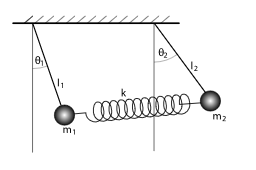
\includegraphics[width=0.5\textwidth]{graphics/gleichsinnig.png}
  \caption{Gleichsinnige Schwingung \cite{Wikipedia}}
\end{figure}

\subsubsection{Die Gegensinnige Schwingung}

Die beiden Pendel werden in entgegengesetze Richtungen ausgelenkt, so dass
gilt :

$\phi_1 = -\phi_2$.

Dadurch wirkt die Feder auf beide Pendel eine gleich große,
entgegengesetzte Kraft aus. Für die Schwingungsfrequenz und die Schwingungsdauer
gilt dann:
\begin{equation}
\label{eqn:omega-}
\omega_-=\sqrt{\frac{g}{l}+\frac{2K}{l}}
\end{equation}
\begin{equation}
\label{eqn:T-}
T_-=\frac{2\pi}{\sqrt{\frac{g}{l}+\frac{2K}{l}}}
\end{equation}
\begin{figure}[H]
  \centering
  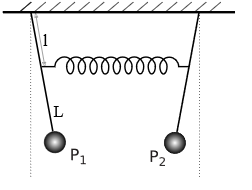
\includegraphics[width=0.5\textwidth]{graphics/gegensinnig.png}
  \caption{Gegensinnige Schwingung \cite{Wikipedia}}
\end{figure}

\subsubsection{Gekoppelte Schwingung und Schwebung}

Jede andere gekoppelte Schwingung lässt sich als Überlagerung dieser beiden
Eigenschwingungen interpretieren. Der Kopplungsgrad lässt sich über die
Schwingungsdauern der gleich- und gegenphasigen Schwingungen berechnen:
\begin{equation}
  \label{eqn:k}
  K = \frac{T_+^2-T_-^2}{T_+^2+T_-^2}.
\end{equation}

Relevant für den Versuch ist neben den
Eigenschwingungen die Schwingung mit den Anfangsbedingungen
$\phi_1 = 0$ und $\phi_2 \neq 0$.
Dabei lässt sich das Phänomen der Schwebung betrachten: Das zu $t = 0$
ausgelenkte Pendel überträgt seine Energie und damit die Schwingungsbewegung
kontinuierlich und vollständig
auf das andere Pendel, bis ersteres stillsteht und letzteres
mit der vollen Amplitude schwingt. Dieser Vorgang wiederholt sich periodisch.
Die Periodendauer dieses Vorgangs wird als Schwebungsdauer $T_s$ bezeichnet und
ist durch die Schwingungsdauern der gleich- und gegenphasigen Schwingungen
gemäß \ref{eqn:Ts} gegeben.
\begin{equation}
  \centering
  T_s  = \frac{T_+ \cdot T_-}{T_+ - T_-}
  \label{eqn:Ts}
\end{equation}

\begin{figure}[H]
  \centering
  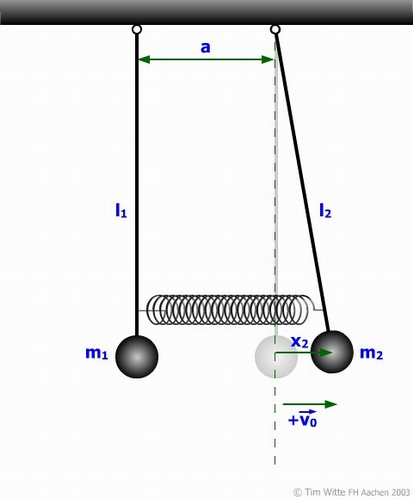
\includegraphics[width=0.5\textwidth]{graphics/gekoppelt.jpg}
  \caption{Gegensinnige Schwingung \cite{fhaachen}}
\end{figure}
